\documentclass[legalpaper,12pt,addpoints]{exam}
\usepackage[utf8]{inputenc}
\usepackage[english]{babel}
\usepackage{graphicx}
\usepackage[none]{hyphenat}
\usepackage[top=1in, bottom=1in, left=0.75in, right=0.75in]{geometry}
\usepackage{amsmath,amssymb}
\usepackage{wrapfig}
\usepackage{comment}
\usepackage{multicol}
\usepackage{multirow}
\usepackage{graphicx}
\usepackage{upgreek} % para poner letras griegas sin cursiva
\usepackage{cancel} % para tachar
\usepackage{mathdots} % para el comando \iddots
\usepackage{mathrsfs} % para formato de letra
\usepackage{stackrel} % para el comando \stackbin
\usepackage{pstricks}
\usepackage{marginnote}
\usepackage{tcolorbox}
\tcbuselibrary{theorems}
\usepackage{circuitikz}
\usepackage{tikz}
\usepackage{pdfpages}

\newcommand{\university}{Universidad del B\'io-B\'io }
\newcommand{\faculty}{Facultad de Ciencias}
\newcommand{\class}{F\'isica II - Electromagnetismo}
%\newcommand{\class}{F\'isica I M\'odulo 2}
\newcommand{\examnum}{\textbf{Certamen 1 REC}}
\newcommand{\content}{Campos Magnéticos por Biot-Savart y Ampere y Ley de Inducción de Faraday Lenz}
%\newcommand{\examdate}{\today}
\newcommand{\examdate}{Abril 9, 2025}
\newcommand{\timelimit}{80 minutos}

\pagestyle{headandfoot}
\firstpageheader{}{}{}
\firstpagefooter{}{Page \thepage\ of \numpages}{}
\runningheader{\class}{\examnum}{\examdate}
\runningheadrule
\runningfooter{}{Page \thepage\ of \numpages}{}
\begin{document}
	
	\pointname{}
	\boxedpoints
	
	\title{
		\begin{center}
			\includegraphics[width=8cm]{figs/cienciasubb.png}\\
			%\Large{\textbf{Certamen 2}}\\
			%Ondas Electromagn'eticas  Ing.Civil El'ectrica UCSC 2021-02\\
		\end{center}
		\class \\  \examnum}
	\date{Octubre 30, 2024}
	\maketitle
	\begin{flushleft}
		\makebox[17cm]{\textbf{Nombre}:\ \hrulefill }\\
		\vspace{1cm}
		\makebox[17cm]{\textbf{Rut}:\ \hrulefill \textbf{Folio}:\ \hrulefill}
	\end{flushleft}
	\noindent \rule{\textwidth}{1pt}
 
\vspace{0.3cm}	
\begin{minipage}[c]{16cm}
    \noindent \textbf{Algunas consideraciones para esta evaluación:}
 \begin{itemize}
 \begin{small}
     \item El certamen 1 contiene \numpages\ páginas (incluida la portada) y \numquestions\ preguntas, con un total de \numpoints puntos.
     \item Cada pregunta debe ser respondida por sólo una respuesta. En caso de presentar más de una, se anulan las respuestas.
     \item No está permitido el uso de celulares o tablet en el desarrollo de esta evaluación. De ser sorprendido utilizando estos artículos su evaluación será califica con nota 1.0.
     \item Buena suerte!
      \end{small}
 \end{itemize}
\end{minipage}
 
 

%%%%%%%%%%%%%% nombre de los profes

\begin{table}[h]
\begin{center}
\begin{tabular}{ccccc}
\multicolumn{5}{l}{\noindent Seleccione con una \textbf{X} el nombre del profesor de su sección:}\\ \cline{1-2} \cline{4-5} 
\multicolumn{1}{|p{5.5cm}|}{Prof. Luis Soto}                      & \multicolumn{1}{p{1.5cm}|}{} & \multicolumn{1}{p{1.0cm}|}{} & \multicolumn{1}{p{5.5cm}|}{Prof. Natalia Molina}     & \multicolumn{1}{p{1.5cm}|}{} \\ \cline{1-2} \cline{4-5} 
\multicolumn{1}{|p{5.5cm}|}{Prof. Evelyn Riveros}                  & \multicolumn{1}{p{1.5cm}|}{} & \multicolumn{1}{p{1.5cm}|}{} & \multicolumn{1}{p{5.5cm}|}{Prof. Ricardo Espinoza}       & \multicolumn{1}{p{1.5cm}|}{} \\ \cline{1-2} \cline{4-5} 
\multicolumn{1}{|p{5.5cm}|}{Prof. Bayron Cerda}                  & \multicolumn{1}{p{1.5cm}|}{} & \multicolumn{1}{p{1.5cm}|}{} & \multicolumn{1}{p{5.5cm}|}{Prof. Cristobal Gatica}       & \multicolumn{1}{p{1.5cm}|}{} \\ \cline{1-2} \cline{4-5} 
%\\ \cline{1-2} \cline{4-5} 
\multicolumn{1}{|p{5.5cm}|}{Prof. Luis Liempi}                  & \multicolumn{1}{p{1.5cm}|}{} & \multicolumn{1}{p{1.5cm}|}{} & \multicolumn{1}{p{5.5cm}|}{}       & \multicolumn{1}{p{1.5cm}|}{} \\ \cline{1-2} \cline{4-5} 
\end{tabular}
\end{center}
\end{table}





	\begin{center}
		\large{
			\textbf{Puntaje}\\
			\medskip
			%\combinedgradetable[v][questions]}
                 \gradetable[v][questions]}
	\end{center}
	
	
	\clearpage
	\begin{questions}

%----------- PROBLEMA 1 --------
 %--------------- Fuerza eléctrica ------------
		%\begin{comment}
\begin{minipage}[c]{10cm}
  \question[19] Un sistema está compuesto de 4 cargas eléctricas puntuales: $q_1=-4[\mu C]$, $q_2=4[\mu C]$, $q_3=8[\mu C]$ y $q_4=2[\mu C]$, dispuestas en el plano cartesiano como se indica en la figura.\\
  Considerando que el valor de la constante de Coulomb es $K=9\times 10^9[Nm^2/C^2]$ y que cada cuadrado de la cuadricula mide $1[cm]$, resuelva:
   \end{minipage}
   %Figura certamen
   \begin{minipage}[c]{6cm}
 % \begin{figure}[H]
    \centering
   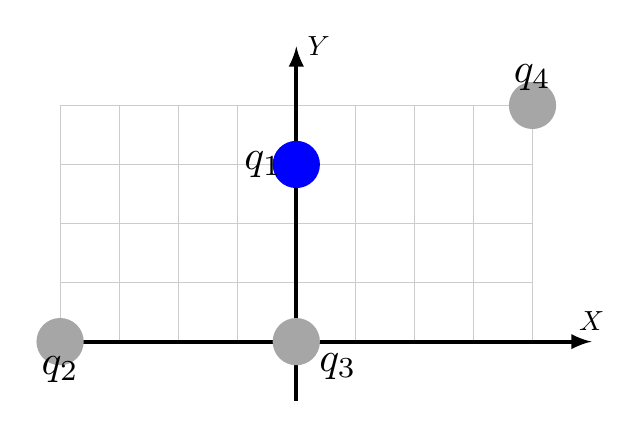
\begin{tikzpicture}[scale=0.750]
  \draw[step=1cm,very thin, gray!40] (-4,0) grid (4,4);
   \draw[black,line width=1.5,->,>=latex, scale=1] (-4,0) -- (5,0) node[black, above, scale=1] {$X$};
   \draw[black,line width=1.5,->,>=latex,scale=1] (0,-1) -- (0,5) node[black, right, scale=1] {$Y$};
   \fill [blue] (0,3) circle (0.4);
 \fill [gray!70] (0,0) circle (0.4);
      \fill [gray!70] (-4,0) circle (0.4);
        \fill [gray!70] (4,4) circle (0.4);
    \node[black,right, scale=1.5, left] at (0,3) {$q_1$};
     \node[black,right, scale=1.5, below] at (-4,0) {$q_2$};
      \node[black,right, scale=1.5, xshift=2pt, yshift=-6pt] at (0,0) {$q_3$};
       \node[black,right, scale=1.5, above] at (4,4) {$q_4$};
   \end{tikzpicture}
   \end{minipage} 
    \begin{parts}
        \part {\bf\red{(3.0 pts)}} Dibuje los vectores de fuerza que actúan sobre la carga $q_3$.
        \part {\bf\red{(12.0 pts)}} Calcule la Fuerza resultante que actúa sobre la carga $q_3$.
        \part {\bf\red{(4.0 pts)}} Suponga que se elimina la carga $q_3$, calcule el campo eléctrico resultante producido por el sistema de cargas en esa posición.
        \end{parts}
 
%\end{comment}

% \begin{comment}
\newpage
%%%%%%%%%%%%%%%%%    PAUTA PROBLEMA 1 %%%%%%%%
\begin{parts}
    \part {\bf\red{(3.0 pts)}}Dibuje los vectores de fuerza que actúan sobre la carga $q_3$.\\
\begin{minipage}[c]{8cm}
La carga $q_3$ interactúa con las cargas $q_1$, $q_2$ y $q_4$. 
Como la carga $q_1$ es negativa al interactuar con la carga positiva $q_4$ la fuerza es atractiva, en cambio, la carga $q_2$ y $q_4$ son positivas al igual que $q_3$,  por lo que la fuerza entre ellas es repulsiva.
    ${\bf \blue{(1.0\ \mbox{pts})}}$ por cada vector.
\end{minipage} 
%    imagen del certamen
 %Figura certamen
   \begin{minipage}[c]{6cm}
 % \begin{figure}[H]
    \centering
   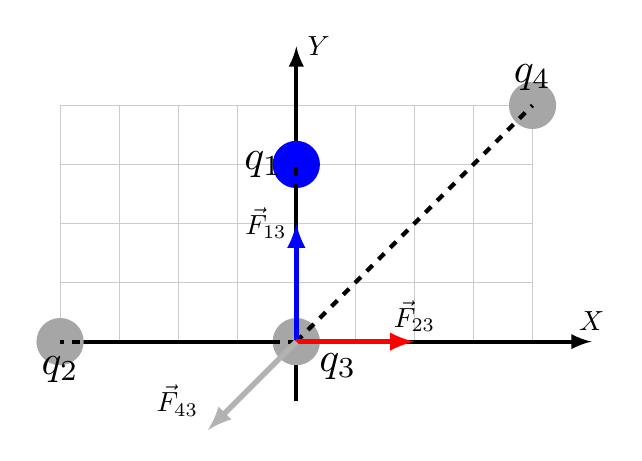
\begin{tikzpicture}[scale=0.750]
  \draw[step=1cm,very thin, gray!40] (-4,0) grid (4,4);
   \draw[black,line width=1.5,->,>=latex, scale=1] (-4,0) -- (5,0) node[black, above, scale=1] {$X$};
   \draw[black,line width=1.5,->,>=latex,scale=1] (0,-1) -- (0,5) node[black, right, scale=1] {$Y$};
   \fill [blue] (0,3) circle (0.4);
 \fill [gray!70] (0,0) circle (0.4);
      \fill [gray!70] (-4,0) circle (0.4);
        \fill [gray!70] (4,4) circle (0.4);
    \node[black,right, scale=1.5, left] at (0,3) {$q_1$};
     \node[black,right, scale=1.5, below] at (-4,0) {$q_2$};
      \node[black,right, scale=1.5, xshift=2pt, yshift=-6pt] at (0,0) {$q_3$};
       \node[black,right, scale=1.5, above] at (4,4) {$q_4$};
        \draw[black,line width=1.5, dashed] (0,0) -- (0,3);
  \draw[black,line width=1.5, dashed] (0,0) -- (-4,0);
  \draw[black,line width=1.5, dashed] (0,0) -- (4,4);
           \draw[blue,line width=2,->, >=latex,scale=1] (0,0) -- (0,2);
           \draw[red,line width=2, ->,>=latex] (0,0) -- (2,0);
           \draw[gray!60,line width=2, ->,>=latex] (0,0) -- (-1.5,-1.5);
 %\draw[gray,line width=1.5, dashed] (0,6) -- (8,6);   
  \node[black,left, scale=1, left] at (0,2) {$\vec{F}_{13}$};
  \node[black,below, scale=1, above] at (2,0) {$\vec{F}_{23}$};
  \node[black,below, scale=1, left] at (-1.5,-1) {$\vec{F}_{43}$};
   \end{tikzpicture}
   \end{minipage} 
   
   \part {\bf\red{(12.0 pts)}} Calcule la Fuerza resultante que actúa sobre la carga $q_3$.
   La fuerza resultante sobre $q_3$ está dada por:
   \begin{align*}
       \vec{F}_3&= \vec{F}_{13}+\vec{F}_{23}+\vec{F}_{43}
   \end{align*}
Cada fuerza se calcula a partir de la ley de Coulomb:
\begin{align*}
       \vec{F}_{ij}&= \frac{K q_i q_j}{||\vec{r}_{ij}||}\vec{r}_{ij}
   \end{align*}
  % Fuerza F13 y vectores de posición carga 1 y 3
 \begin{minipage}[c]{4cm}
 % \begin{figure}[H]
    \centering
   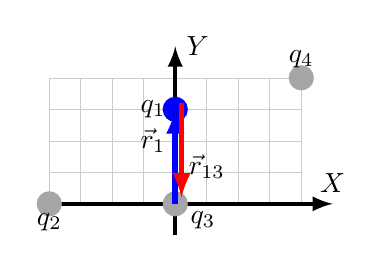
\begin{tikzpicture}[scale=0.40]
  \draw[step=1cm,very thin, gray!40] (-4,0) grid (4,4);
   \draw[black,line width=1.5,->,>=latex, scale=1] (-4,0) -- (5,0) node[black, above, scale=1] {$X$};
   \draw[black,line width=1.5,->,>=latex,scale=1] (0,-1) -- (0,5) node[black, right, scale=1] {$Y$};
   \fill [blue] (0,3) circle (0.4);
 \fill [gray!70] (0,0) circle (0.4);
      \fill [gray!70] (-4,0) circle (0.4);
        \fill [gray!70] (4,4) circle (0.4);
    \node[black,right, scale=1, left] at (0,3) {$q_1$};
     \node[black,right, scale=1, below] at (-4,0) {$q_2$};
      \node[black,right, scale=1, xshift=2pt, yshift=-6pt] at (0,0) {$q_3$};
       \node[black,right, scale=1, above] at (4,4) {$q_4$};
        \draw[black,line width=1.5, dashed] (0,0) -- (0,3);
 % \draw[black,line width=1.5, dashed] (0,0) -- (-4,0);
 % \draw[black,line width=1.5, dashed] (0,0) -- (4,4);
           \draw[blue,line width=2,->, >=latex,scale=1] (0,0) -- (0,3);
           \draw[red,line width=2, ->,>=latex] (0.2,3.2) -- (0.2,0.2);
         %  \draw[gray!60,line width=2, ->,>=latex] (0,0) -- (-1.5,-1.5);
 %\draw[gray,line width=1.5, dashed] (0,6) -- (8,6);   
  \node[black,left, scale=1, left] at (0,2) {$\vec{r}_{1}$};
  \node[black,below, scale=1, above] at (1,0.5) {$\vec{r}_{13}$};
  %\node[black,below, scale=1, left] at (-1.5,-1) {$\vec{F}_{43}$};
   \end{tikzpicture}
   \end{minipage} 
 \begin{minipage}[c]{12cm}
 \begin{align*}
     \vec r_1+\vec{r}_{13}=\cancelto{\vec{0}}{\vec{r}_{3}} \implies \vec{r}_{13}&=-\vec{r}_1\\
     \vec{r}_{13}&=-0,03\hat{y}[m] \ \ {\blue{(0.5\ \mbox{pts})}} \\\therefore ||\vec{r}_{13}||&=0.03[m] \ \ {\blue{(0.5\ \mbox{pts})}}\\
     \therefore \vec{F}_{13}&=\frac{9\times 10^9[Nm^2/C^2] (-4\times 10^{-6}[C]) (8\times 10^{-6})}{(3\times 10^{-2}[m])^2}(-\hat{y})\\
    \vec{F}_{14}&= 320\hat{y}[N] \ \ {\blue{(2.0\ \mbox{pts})}}
     \end{align*}
 \end{minipage}
     % Fuerza F23 y vectores de posición carga 2 y 3
  \begin{minipage}[c]{4cm}
      \begin{minipage}[c]{4.5cm}
 % \begin{figure}[H]
    \centering
   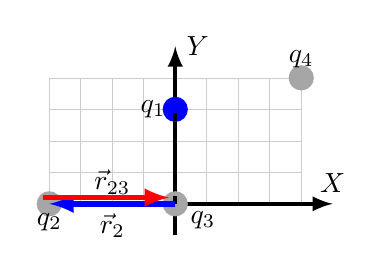
\begin{tikzpicture}[scale=0.40]
  \draw[step=1cm,very thin, gray!40] (-4,0) grid (4,4);
   \draw[black,line width=1.5,->,>=latex, scale=1] (-4,0) -- (5,0) node[black, above, scale=1] {$X$};
   \draw[black,line width=1.5,->,>=latex,scale=1] (0,-1) -- (0,5) node[black, right, scale=1] {$Y$};
   \fill [blue] (0,3) circle (0.4);
 \fill [gray!70] (0,0) circle (0.4);
      \fill [gray!70] (-4,0) circle (0.4);
        \fill [gray!70] (4,4) circle (0.4);
    \node[black,right, scale=1, left] at (0,3) {$q_1$};
     \node[black,right, scale=1, below] at (-4,0) {$q_2$};
      \node[black,right, scale=1, xshift=2pt, yshift=-6pt] at (0,0) {$q_3$};
       \node[black,right, scale=1, above] at (4,4) {$q_4$};
        \draw[black,line width=1.5, dashed] (0,0) -- (0,3);
 % \draw[black,line width=1.5, dashed] (0,0) -- (-4,0);
 % \draw[black,line width=1.5, dashed] (0,0) -- (4,4);
           \draw[blue,line width=2,->, >=latex,scale=1] (0,0) -- (-4,0);
           \draw[red,line width=2, ->,>=latex] (-4.2,0.2) -- (-0.2,0.2);
         %  \draw[gray!60,line width=2, ->,>=latex] (0,0) -- (-1.5,-1.5);
 %\draw[gray,line width=1.5, dashed] (0,6) -- (8,6);   
  \node[black,left, scale=1, below] at (-2,0) {$\vec{r}_{2}$};
  \node[black,below, scale=1, above] at (-2,0) {$\vec{r}_{23}$};
  %\node[black,below, scale=1, left] at (-1.5,-1) {$\vec{F}_{43}$};
   \end{tikzpicture}
   \end{minipage} 
  \end{minipage}
 \begin{minipage}[c]{12cm}
 \begin{align*}
     \vec r_2+\vec{r}_{23}=\vec{r}_{3} \implies \vec{r}_{23}&=\cancelto{\vec{0}}{\vec{r}_3}-\vec{r}_2\\
     \vec{r}_{24}&=0,04\hat{x}[m] \ \ {\blue{(0.5\ \mbox{pts})}} \therefore ||\vec{r}_{23}||=0,04[m] \ \ {\blue{(0.5\ \mbox{pts})}} \\
     \therefore \vec{F}_{24}&=\frac{9\times 10^9[Nm^2/C^2] (4\times 10^{-6}[C]) (8\times 10^{-6})}{(4\times 10^{-2}[m])^2}\hat{x}\\
    \vec{F}_{24}&=180\hat{x}[N] \ \ {\blue{(2.0\ \mbox{pts})}}
 \end{align*}
 \end{minipage}
%%%% Fuerza F34 y vectores de posicion cargas 3 y 4
  \begin{minipage}[c]{4.3cm}
     \begin{minipage}[c]{4cm}
      \begin{minipage}[c]{4.5cm}
 % \begin{figure}[H]
    \centering
   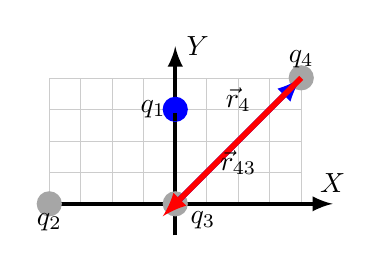
\begin{tikzpicture}[scale=0.40]
  \draw[step=1cm,very thin, gray!40] (-4,0) grid (4,4);
   \draw[black,line width=1.5,->,>=latex, scale=1] (-4,0) -- (5,0) node[black, above, scale=1] {$X$};
   \draw[black,line width=1.5,->,>=latex,scale=1] (0,-1) -- (0,5) node[black, right, scale=1] {$Y$};
   \fill [blue] (0,3) circle (0.4);
 \fill [gray!70] (0,0) circle (0.4);
      \fill [gray!70] (-4,0) circle (0.4);
        \fill [gray!70] (4,4) circle (0.4);
    \node[black,right, scale=1, left] at (0,3) {$q_1$};
     \node[black,right, scale=1, below] at (-4,0) {$q_2$};
      \node[black,right, scale=1, xshift=2pt, yshift=-6pt] at (0,0) {$q_3$};
       \node[black,right, scale=1, above] at (4,4) {$q_4$};
        \draw[black,line width=1.5, dashed] (0,0) -- (0,3);
 % \draw[black,line width=1.5, dashed] (0,0) -- (-4,0);
 % \draw[black,line width=1.5, dashed] (0,0) -- (4,4);
           \draw[blue,line width=2,->, >=latex,scale=1] (0,0) -- (4,4);
           \draw[red,line width=2, ->,>=latex] (4,4) -- (-0.4,-0.4);
         %  \draw[gray!60,line width=2, ->,>=latex] (0,0) -- (-1.5,-1.5);
 %\draw[gray,line width=1.5, dashed] (0,6) -- (8,6);   
  \node[black,left, scale=1, below] at (2,4) {$\vec{r}_{4}$};
  \node[black,below, scale=1, below] at (2,2) {$\vec{r}_{43}$};
  %\node[black,below, scale=1, left] at (-1.5,-1) {$\vec{F}_{43}$};
   \end{tikzpicture}
   \end{minipage} 
  \end{minipage}
  \end{minipage}
 \begin{minipage}[c]{12cm}
 \begin{align*}
     \vec r_4+\vec{r}_{43}&=\vec{r}_{3} \implies \vec{r}_{43}=\cancelto{\vec{0}}{\vec{r}_3} -\vec{r}_4 = (-0,04\hat{x} - 0,04\hat{y})[m] \ \ {\blue{(0.5\ \mbox{pts})}}\\ \therefore ||\vec{r}_{43}||&=0,04\sqrt{2}[m] \ \ {\blue{(0.5\ \mbox{pts})}}
      \end{align*}
      \begin{align*}
     \therefore \vec{F}_{43}&=\frac{9\times 10^9[Nm^2/C^2] (2\times 10^{-6}[C]) (8\times 10^{-6})}{(4\sqrt{2}\times 10^{-2}[m])^3}(-4\times 10^{-2}\hat{x} - 4\times 10^{-2}\hat{y})\\
    \vec{F}_{43}&=\frac{90\times 10^{-3}}{2\sqrt{2}\times 10^{-4}} (-\hat{x} - \hat{y})[N]=-31,82(\hat{x} +\hat{y})[N]\approx -32 (\hat{x} +\hat{y})[N] \\ 
		{\blue{(2.0\ \mbox{pts})}}
 \end{align*}
 \end{minipage}
Finalmente la fuerza sobre la carga $q_3$:
\begin{align*}
    \vec{F_3}=(180-32)\hat{x}+(320-32)\hat{y}=(148\hat{x}+288\hat{y})[N] \ \ {\blue{(3.0\ \mbox{pts})}}
\end{align*}
 
% pregunta C

  \part {\bf\red{(4.0 pts)}} Suponga que se elimina la carga $q_3$, calcule el campo eléctrico resultante producido por el sistema de cargas en esa posición.
 Dado que conocemos la fuerza eléctrica sobre la carga $q_3$, podemos calcular el campo eléctrico en esa posición mediante la relación $$\vec{E}=\frac{\vec{F}}{q} \ \ {\blue{(1.0\ \mbox{pts})}}$$
\begin{align*}
    \vec{E}&=\frac{\vec{F}}{q}=\frac{(148\hat{x}+288\hat{y})[N]}{8\times 10^{-6}[C]}\\
    &=(18,5\hat{x} +36\hat{y})\times 10^6 [N/C]\ \ {\blue{(3.0\ \mbox{pts})}}
\end{align*}
\end{parts}


%\end{comment}


%----------------------------------------------
%%%%%%%%%%%%%%%%% PROBLEMA 2 %%%%%%%%%%%%%%%%%%%%%%%%%%
%--------- campo elèctrico cargas puntuales ------------------------%	
%----------------------------------------------

\newpage
%\begin{comment}
\begin{minipage}[c]{0.6\textwidth}
  \question[20]xxxx
  \begin{parts}
        \part {\bf\red{(5.0 pts)}}xxxx.
        \part {\bf\red{(10.0 pts)}} xxx.
        \part {\bf\red{(5.0 pts)}} xxxx.
        \end{parts}
        
   \end{minipage}   
\begin{minipage}[c]{0.4\textwidth}
\begin{center}
%\includegraphics[scale=0.25]{figs/Campo.jpg}
\end{center} 
\end{minipage}


%\end{comment}	
		

%----------------------------------------------
%%%%%%%%%%%%%%%%% PROBLEMA 3 %%%%%%%%%%%%%%%%%%%%%%%%%%
%--------- distribuciones de carga ------------------------%	
%----------------------------------------------

\newpage
%\begin{comment}
\begin{minipage}[c]{11cm}
  \question[20] xxx
 
\end{minipage}
\begin{minipage}[c]{7cm}
%\includegraphics[scale=0.070]{figs/fig-control1.png}
\end{minipage}\\
\begin{parts}

\part  {\bf\red{(12.0\ pts)}} xxx\\


\part {\bf\red{(8.0\ pts) }} xxx\\
        \end{parts}



%\end{comment}		


% \begin{comment}
%\newpage
  % \includepdf[pages=1-4]{PAUTA-C1_REC_ICE_UBB_S2_2024.pdf}
%\end{comment}
		
	
	\end{questions}
\end{document}
